\documentclass{beamer}

\usepackage{tikz}
\usepackage{tikzlings}
\usepackage{tikzducks}


\setbeamertemplate{background canvas}{
	\begin{tikzpicture}[remember picture, overlay]
	\node at (current page.center) {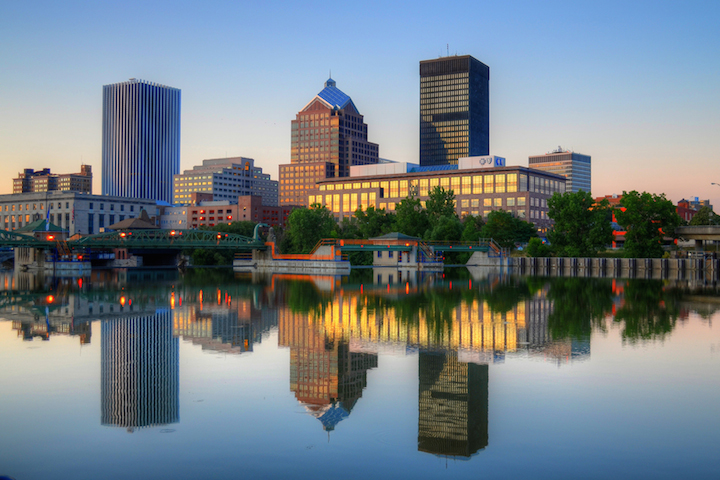
\includegraphics[height=1\paperheight]{Rochester}};
	\end{tikzpicture}
}
\setbeamertemplate{navigation symbols}{}

\begin{document}
	
\begin{frame}<1->
	\begin{tikzpicture}[remember picture, overlay]
		\node[fill=white,yshift=-1cm,inner sep=8pt] at (current page.north) {\large TUG'20 -- Rochester -- summer 2020};
%		\duck[scale=1.2,xshift=7cm,yshift=-2.8cm]
%		\bear[scale=1.3,xshift=5.5cm,yshift=-2.7cm]
%		\snowman[scale=1.2,xshift=4cm,yshift=-3cm]
%		\node[at=(current page.center),yshift=-4cm] {
\includegraphics[width=\paperwidth]{conveyor}};
%		\node at (31-0.1*\thepage,-2) {
\includegraphics[height=3cm]{Packages}};
%		\draw[lightgray!90!black,line width=5pt] (0,-3.5) rectangle ++(1.8,2);
%		\fill[lightgray!90!black] (-0.08,-1.5) rectangle ++(1.96,1);
%		\node<3-6,32-36,92-95,121-125,151-154,181-184,240-243,269-273,299-303,329-333,359-362,418-421,448-451,477-481>[fill=green, text width=1.4cm,align=center] at (0.92,-1) {OK};
%		\node<62-66,210-214,388-392>[fill=red, text width=1.4cm,align=center] at (0.92,-1) {FAIL};
%		\node[at=(current page.south),yshift=0.2cm]{%
%		\tiny\color{white}Background: \url{https://commons.wikimedia.org/wiki/File:Factory_and_industrial_management_(1891)_(14758513856).jpg}};
%	\end{tikzpicture}
%	\pause[489]
%\end{frame}	
%
%\begin{frame}<1->
%	\begin{tikzpicture}[remember picture, overlay]
%		\node[fill=yellow!10!white,yshift=-1cm,draw=lightgray!90!black,line width=4pt,inner sep=8pt] at (current page.north) {\Huge CTAN package checking};
%		\duck[scale=1.2,xshift=7cm,yshift=-2.8cm]
%		\bear[scale=1.3,xshift=5.5cm,yshift=-2.7cm]
%		\snowman[scale=1.2,xshift=4cm,yshift=-3cm]
%		\node[at=(current page.center),yshift=-4cm] {
\includegraphics[width=\paperwidth]{conveyor}};
%		\node at (31-0.1*489,-2) {
\includegraphics[height=3cm]{Packages}};
%		\draw[lightgray!90!black,line width=5pt] (0,-3.5) rectangle ++(1.8,2);
%		\fill[lightgray!90!black] (-0.08,-1.5) rectangle ++(1.96,1);
		\node[at=(current page.south),yshift=0.2cm]{%
		\tiny\color{white}Background: \url{https://commons.wikimedia.org/wiki/File:Downtown_Rochester,_NY_HDR_by_patrickashley.jpg}};
	\end{tikzpicture}
%	\pause[50]
\end{frame}	
	
\end{document}